\chapter{Methodology}
\label{chap:meth}

This chapter starts with the analysis of requirements for the implemented
software. In the second section of the chapter I will discuss possible
approaches to adapt an external state machine to Phantom OS persistency model.
The last section describes the implementation and design decisions in detail.

\section {Requirements analysis}

As previous chapters of this paper suggest, the goal of this paper is to create
an implementation of a TCP suitable for a persistent system. More precisely, I
target a port of Phantom OS to Genode OS framework. This section contains a
list of requirements that I will follow while designing my own protocol
implementation.

\subsection {Transparency for client applications}
Persistent support systems (PSSs) aim to make development of applications
easier. The PSSs provide their clients with an abstraction of an uninterrupted
execuiton. In a real world, however, a computer system may experience
downtimes. The point of a PSS is to hide these downtimes from applications that
use it. Such hiding of undesired effects is generally called
\textit{transparency}.

As discussed in Section \ref{sec:int:phantom}, the current implementation of
networking stack is not transparent for the applications residing in PVM.
Application designers should foresee existence of these errors and write
handlers for them. To make PoG port really orthogonally persistent these errors
should be hadled at PSS level, not by clients.

That means that the state of TCP connections should be the same before a
shutdown and after a reboot. To achieve that a persistent TCP implementation
should either (1) backup and restore connections state or (2) make the
disappearance of a remote peer invisible for application on the other end of
the connection. Of course, restoration of the state should be done before
returning control to applications.

(1) can be achieved with reestablishing connections on startup. However, the
remote peer should be ready to the reestablishment request. This is problematic
in case when a persistent host plays role of a server in a client-server
communication. (2) can be achieved with use of an message broker that will
mimic an alive host with full TCP input queue. Thus it will keep the connection
alive but prohibit sending packets to the channel. Another way to achieve (2)
is to send a control message to the remote socket. The remote TCP in this case
should efficiently do the same thing as a message broker did. It should mimic
live connection that cannot accept data. The drawback of this approach is that
to exchange control messages both communicating peer should have enhanced TCP
stack.

\subsection {Robustness to rollbacks}

Phantom OS uses full-memory snapshots of PVM memory space to provide
persistence for its clients. Snapshots are taken in a live mode so that
processes inside the VM continue to run. Due to the two previous facts,
computational operations of PVM applications can be executed more than once.
For example, assume that an application receives packets A, B, and C.  Assume
that after packet A is received, snapshot is performed. While it was on
progress, the application receives packet B. After the snapshot was made,
applications reveives packet C and immediately after this machine goes down.
After the snapshot would be restored the application will have no knowledge
that it already received packets B and C. Thus the application will send ACK
packet for A, which will result in error because the remote peer does not
expect this ACK. Moreover, it is unable to retransmit this packet, since it is
not exist in remote TCP's retransmission queue, because it was already
acknowledged when the application received B and C.

Phantom OS snapshot mechanism takes into account that snapshot is not a atomic
process. Thus, in usual case it would handle reception of packet B properly,
i.e. the client application would know that B was received. But in case of 
PoG the TCP stack is not stateless like Phantom kernel but still transient.
Therefore, if TCP receives a packet but does not passes it to the application
before restart, this packet may be lost. The remote peer expects that the
application processed it but the application never received it because TCP did
not finish delivering it to the application.

Three solutions exist that may solve the problem above. The first is to refrain
from sending acknowledgment packets if a received packet is not included in any
snapshot. However, this will either dramatically increase the number of
retransmissions in a network, which will result in reduced network performance
or it will require doing snapshots very often. In such case a snapshot should
be performed each 50ms to avoid extra network congestion at all. However, in
PoG a snapshot runs for around 10 seconds. This approach is not acceptable with
such a long snapshot.  

The second solution is to keep in persistent memory a buffer that will store
all packets that TCP clients had not consumed yet. In this case persistent
memory can be a regular file or snapshotted memory space. 

The third approach is to have a message broker inside a network that will
function similarly to the buffer in the second approach. The broker can save
all acknowledged packets in a network, and flush its queue when it detects that
receiving host has done a snapshot. ICMP messages or some similar stateless
network protocol could be useful to notify the broker about the end of the
snapshot process.

\subsection {Usefullness}

Phantom OS is already capable of restoring sockets in CLOSED and LISTEN states.
For a Genode implementation of a persistent TCP to be useful it should work for
the same or bigger set of states. Even if the developed software will only
support the same set of states the fact that the software is implemented as a
Genode component will greatly improve maintainablility of the software.

\subsection {Compatibility with existing protocols}

The last design goal is not directly related to providing persistent I/O
abstraction to the clients of a network stack. Since snapshotting is a very
popular technique for implementing persistent systems, and Genode is actively
used to develop various operating systems, it is probable that some other
developers might want to use persistent TCP in their software.

That means that result of this work should be a standalone application that
works without Phantom and is flexible enough to support all use cases that may
arise. Fortunately, Genode's component-based architecture helps greatly with
it. Another reason to make persistent TCP implementation a standalone
application is that the PoG port is not yet ready for me to experiment with it.

Another thing that should be addressed in the design of the API of the system,
is easy migration from non-persistent TCP stacks that are already available in
Genode, namely lwip and lxip. To do this I intend to design API very similar to
regular sockets or even exactly the same, but with different call semantics. I
also plan to add a Virtual File System (VFS) plugin that will expose sockets as
regular files because this is the way how Genode developers suggest
integrating sockets into the Genode ecosystem since version 18.11. With such
implementation, even relinking of existing binary will be not needed. The only
thing user would need is to change the configuration of the init Genode
component.

\section{On persisting of finite state machines}

Most TCP implementations implement logical state of the sockets as finite state
machines. Since the goal of the paper is to create a persistent TCP
implementation, it might be useful to consider how an arbitrary FSM can be
snapshotted to restore it later to the same state from the snapshot. 

The most straightforward and universal way to achive the desired outcome is to
use a full-memory snapshot of a running process. Full-memory snapshot should
include stack and address space. Also it should include current context, i.e.
general-purpose registers and the program counter. Obtained snapshot should be
stored in a persistent memory and loaded to the apropriate memory on restore.
In principle, this approach would work for any running process.

The second approach is to directly access current state of the FSM. Usually FSM
are implemented on C and C++ as structs or classes holding current state as an
value of an enumerable type. If it is possible to access these structures
directly, simple saving and loading them would work. In some cases, for example
sockets, there are several state machines: one per socket. In such cases FSMs
should be registered at the supervisor that controls inputs and stores FSM
structures.

The last approach requires knowing of internal functioning of an FSM. When all
states and transitions of FSM are known in advance, it is possible to implement
FSM with the same transitions. When the tracking FSM is provided with the same
inputs as the target one states of both FSMs should be in sync. Assessing state
of the tracking FSM will allow observer to determine state of the target FSM.
Moreover, tracking of inputs greatly helps in restoration phase. To restore
state of the target FSM it is enough to provide it with the same inputs once
again. This approach is useful when an FSM does not have a centralized state or
when it cannot be easily accessed.

\section{Implementation process}

I have chosen to implement a persistent TCP stack in form of a Genode component
that will serve as a plugin for a VFS. The users of the TCP stack should add
signal handlers to their components for signals of type SIG\_SNAP and
SIG\_RESTORE. When SIG\_SNAP is received, it is passed to the persistent TCP VFS
plugin which gathers data that should be saved into persistent memory and calls
filesystem service to save socket snapshot structure into persistent memory.

Symmetrically, when SIG\_RESTORE is received, the component will access the
previously saved file and read information about sockets state at the snapshot
moment.

The exact structure of the data needed for the connection restore process and
some conditions for successful persistence of sockets will be discussed in the
following sections of this chapter.

\subsection{Snapshot structure}

As discussed earlier, I decided to make a TCP stack persistent using periodic
snapshotting.  To be useful in process of restoring the state, the snapshot
should indeed have some data stored in it. The content of the snapshot is
discussed in detail in this section.

When deciding about snapshot structure, two distinct approaches exist. The first one is to make a full-memory snapshot, saving each page of virtual
memory into persistent memory. To make snapshot consistent, all threads that use
these memory pages should be stopped, or writing to the pages should be
prohibited.  One of the disadvantages of this type of snapshot is that it is not userspace
friendly, since memory pages are usually managed in the kernel. The last
downside is its relatively big size, in terms of hundreds of megabytes. 

The second approach is to use selective snapshotting. In this case, when the
component forms a snapshot, it should first read certain set of state variables
from memory then serialize them together. After that, the serialized structure
is persisted. The benefits of this approach are easier implementation, and the
smaller size of the snapshot structure. The smaller snapshot size leads to the faster
snapshot/restore process.

I have chosen the second approach. Currently, Genode does not support
full-memory snapshotting, and implementing it from scratch is almost
impossible. Though it may be possible to mimic a full memory snapshot for a
single component by persisting all its dataspaces, it poses additional
challenges. For example, a dataspace might be shared with other components that
are not persisted. In this case persistent component expects its sibling to
write something to the dataspace they used for memory-mapped communication
earlier, and the sibling is unaware of any communications before power loss.

To snapshot socket state selectively, I needed to decide which data needs
to be saved. 

\begin{figure}
    \centering
    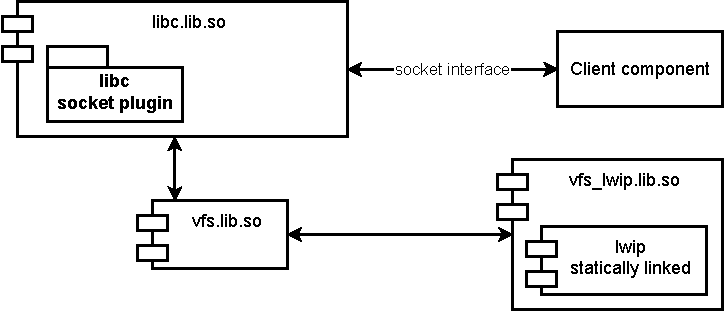
\includegraphics[]{figs/vfs_components.drawio.pdf}
    \caption{Control path of socket API}
    \label{fig:socket_via_vfs}
\end{figure}

Figure \ref{fig:socket_via_vfs} shows all libraries that are related to the
socket interface. To find out, which of them contain state that needs to be
snapshotted I have studied their source codes and how their clients should use
them. 

The libc is the library that provides a libc runtime and API for client
applications. Part of the standard libc API is a socket API. It includes
well-known functions socket(), bind(), listen(), and others. Genode libc
implementation is based upon a FreeBSD libc with some adjustments. In this
library socket API is implemented as a libc plugin. Libc plugin is a logically
independent part of code, responsible for a single API. In this case, it is
sockets API.  

Libc socket plugin maintains a single Socket\_fs::Context structure per each
created socket. This structure encapsulates a socket state variable \_state,
which is used to determine which calls on the socket are allowed in the current
state. The Context also has \_fd\_flags variable, which represents flags set on
socket. To make the behavior of the plugin consistent after restore, the \_state
and \_fd\_flags variables should be restored.

Internally the libc plugin uses VFS to provide its functionality. VFS is
implemented in form of a shared library, vfs.lib.so. This library is not
interesting from point of snapshotting, as it does not contain any state
itself.  The library in our case is just a proxy and a dynamic loader for VFS
plugins.

State of vfs\_lwip.lib.so should certainly be snapshotted, as this library
contains information required for operation of the TCP itself. Information is
stored in form of Protocol Control Blocks (PCBs). PCB is a structure used at a
protocol level that holds all the data needed for the protocol stack socket
uses. More details about PCBs can be found at \cite{stevens1996tcp}. Each
socket corresponds to exactly one PCB. Fortunately, it seems to be enough to
save the states of all PCBs and then restore them.

\subsection{Snapshot location}

The goal of this paper is to design a persistent networking stack suitable for
Phantom OS. Due to this, it is possible to include a snapshot of the TCP stack
into the Phantom VM snapshot structure. However, I decided that a persistent
network stack can be useful not only for the Phantom OS but also for other
persistent systems. These systems can use other mechanisms for persistence. Due
to this, I decided to make an abstract interface that has functions for saving
and loading binary data from persistent memory.

For simplicity, the only implementation of this service saves its state
directly to the hard drive volume attached to VM. An implementation that saves
and loads data using the Phantom snapshotting mechanism is currently in
progress.

/subsection{Approach with memory}
As a first approach I tried to save memory pages that belong to network stack and 
restore them on booting. At first I tried to snapshot the whole virtual address
space of the component that uses network stack. However, this was problematic
due to the nature of data inside a components' virtual memory. The problem was
with kernel capabilities -- they are used throughout almost each part of the OS
framework. In fact, the component can not exist without using at least one
capability, and can not execute any code without using at least three - namely 
Parent, CPU and RAM capabilities. This ubiquity of the capabilities and the fact
that they become invalid after restart make straightforward dumping of full
component's address space to disk impossible.

The idea of using a proxy that will mask sequence numbers was inspired by
proposal of using packet filters (see rocks-racks).
